\documentclass[12pt]{article}
\usepackage[colorinlistoftodos]{todonotes}
\usepackage{amsmath}
\usepackage{amssymb}
\usepackage{bm}
\usepackage{enumerate}
\usepackage{fancyvrb}
\usepackage[top=1in, bottom=1in, left=1in, right=1in]{geometry}
\usepackage{hyperref}
\hypersetup{
    colorlinks=true,
    linkcolor=blue,
    filecolor=magenta,      
    urlcolor=cyan,
}
\usepackage{placeins}
\usepackage{tikz}
\usepackage{tikzsymbols}
\usepackage{todonotes}
\usepackage{bbm}
\usepackage{color}
\usepackage{mathrsfs}
\usepackage{enumitem}

% \renewcommand{\theenumi}{\roman{enumi}}
\newcommand{\rmn}[1]{{\textcolor{blue}{\bf [{\sc rmn:} #1]}}}
\DeclareMathOperator*{\argmax}{arg\,max}

\usetikzlibrary{positioning,calc}
%%%%%%%%%
\usepackage[most]{tcolorbox}
\newtcolorbox[]{solution}[1][]{%
    breakable,
    enhanced,
    colback=white,
    title=Solution,
    #1
}
%%%%%%%%%%
\title{10-403 Deep Reinforcement Learning and Control\\
  Homework 5: Advanced Policy Gradients\\
  Spring 2019\\
}

\date{March 29th, 2019\\
  \hspace{1cm}\\
Due by 11:59 PM on April 15th, 2019}

\begin{document}

\maketitle
\noindent
\section*{Instructions}

You may work in teams of \textbf{2} on this assignment. Only one person should submit the writeup on Gradescope. Additionally, the same person who submitted the writeup to Gradescope must upload the code to Autolab.  Make sure you mark your partner as a collaborator on Gradescope (you do not need to do this in Autolab) and that both names are listed in the writeup.  Writeups should be typeset in \LaTeX and submitted as PDF. All code, including auxiliary scripts used for testing, should be submitted with a README.  Please limit your writeup to 8 pages or less (excluding the provided instructions).

We've provided some code templates that you can use if you wish. Abiding to the function signatures defined in these templates is not mandatory; you can write your code from scratch if you wish. You can use any deep learning package of your choice (e.g., Keras, Tensorflow, PyTorch). You should not need the cluster or a GPU for this assignment. The models are small enough that you can train on a laptop CPU.

It is expected that all of the work you submit is your own. Submitting a classmate's code or code which copied from online and claiming it is your own is not allowed. Anyone who does this will be violating University policy, and risks failure of the assignment, course and possibly disciplinary action taken by the university.

\section*{Environment}
You are provided with a custom environment in \texttt{2Dpusher\_env.py}.  In order to make the environment using \texttt{gym}, you can use the following code:
\begin{quote}
\begin{verbatim}
import gym
import envs

env = gym.make('Pushing2D-v0')
\end{verbatim}
\end{quote}
Then you can interact with the environment as you usually do.

An overview of the environment is available in the \href{https://docs.google.com/presentation/d/1ueiyyXN_v7h_4GGa4NtMBau0Du1wpZstS3pfJIds37U/edit?usp=sharing}{recitation slides}.  The environment is considered ``solved'' once the percent successes (i.e., the box reaches the goal within the episode) reaches $95\%$. 



\section*{Problem 1: Deep Deterministic Policy Gradients (DDPG) \textbf{[40 pts]}}
\ \\


Previously, in Homework 3, you worked with Deep Q-networks, which is an off-policy method for discrete spaces that learns the actual value of actions given a certain state and then acts greedily with respect to the learned values.  Then, in Homework 4, you implemented on-policy policy gradient methods that learn a good policy directly over a discrete action space.  In this section, you will implement DDPG, an off-policy policy gradient method for a continuous action space.  Similar to DQN, you will 
\begin{enumerate}
    \item use a replay buffer from which you will sample transitions in order to learn off-policy and minimize correlations between samples
    \item train with a slowly updated target Q network to give consistent targets when performing the temporal difference backups
\end{enumerate}
However, since this is a policy gradient method, you will be learning a policy directly, instead of learning Q-values and then acting greedily.

The DDPG algorithm is shown in Figure~\ref{fig:ddpg}.
There are a few things to note:
\begin{enumerate}
    \item Similar to DQN, there are two sets of weights: $\{\theta^{Q},\theta^\mu\}$ are trained and target weights $\{\theta^{Q'}, \theta^{\mu'}\}$ are slowly updated towards the trained weights.  
    \item The algorithm requires a random process $\mathcal{N}$ to offset the deterministic actor policy.  For this assignment, you can use an $\epsilon$-normal noise process, where with probability $\epsilon$, you sample an action uniformly from the action space and otherwise sample from a normal distribution with the mean as indicated by your actor network and standard deviation as a hyperparameter.  
    \item There is a replay buffer $R$ which can have a burn-in period, although this is not required to solve the environment.
    \item The target values values $y_i$ used to update the critic network is a one-step TD backup where the bootstrapped $Q$ value uses the slow moving target weights $\{\theta^{\mu'},\theta^{Q'}\}$.
    \item The update for the actor network differs from the traditional score function update used in vanilla policy gradient.  Instead, DDPG uses information from the critic about how actions influence value estimates and pushes the policy in a direction to maximize increase in estimated rewards.  
\end{enumerate}

\begin{figure}[h]
    \centering
    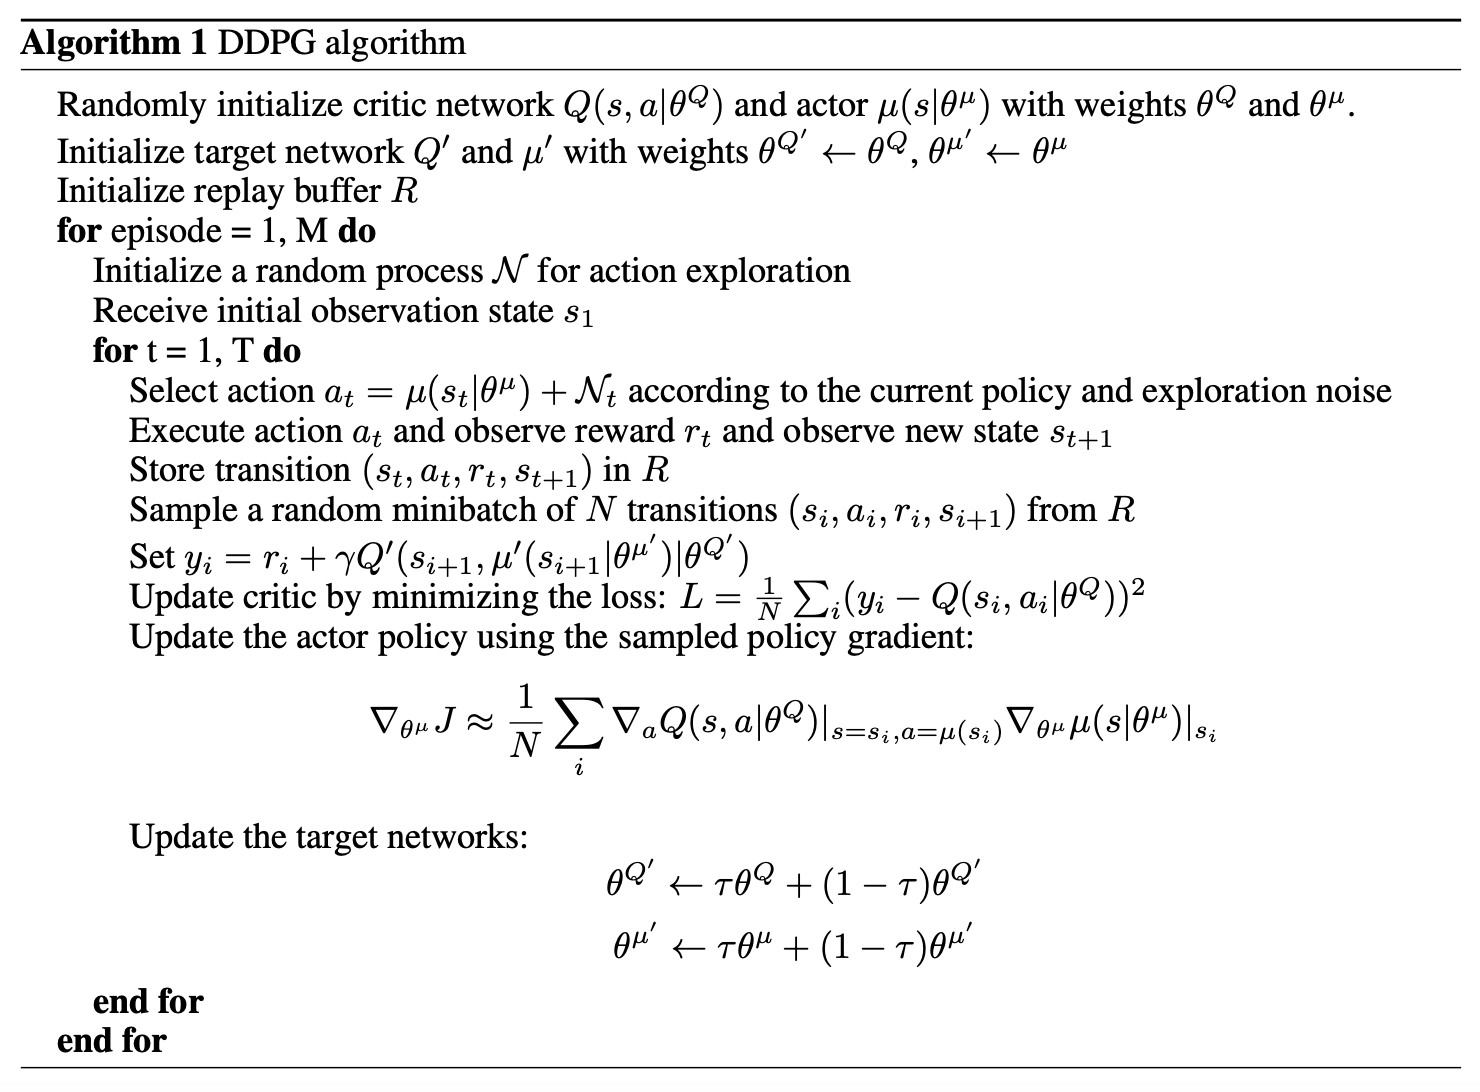
\includegraphics[width=1\textwidth]{ddpg}
    \caption{DDPG algorithm presented by \cite{DBLP:journals/corr/LillicrapHPHETS15}.}
    \label{fig:ddpg}
\end{figure}

For this environment, a simple fully connected network with 2 layers should suffice.  You can choose which optimizer and hyperparameters to use, so long as you are able to solve the environment. We recommend using Adam as the optimizer. It will automatically adjust the learning rate based on the statistics of the gradients it's observing. Think of it like a fancier SGD with momentum. 

Train your implementation on the \texttt{Pushing2D-v0} environment until convergence\footnote{\texttt{Pushing2D-v0} is considered solved if your implementation can reach the goal at least 95\% of the time.}, and answer the following questions:

\begin{enumerate}
\item Describe your implementation, including the optimizer and any hyperparameters you used (learning rate, $\gamma$, etc.).
 \begin{solution}
\end{solution}
\item  Plot the learning curve: Every $k$ episodes, freeze the current cloned policy and run 100 test episodes, recording the mean/std of the cumulative reward. Plot the mean cumulative reward $\mu$ on the y-axis with $\pm \sigma$ standard deviation as error-bars vs. the number of training episodes.  You don't need to use the noise process $\mathcal{N}$ when testing.

Hint: You can use matplotlib's \texttt{plt.errorbar()} function. \url{https://matplotlib.org/api/\_as\_gen/matplotlib.pyplot.errorbar.html}
 \begin{solution}
\end{solution}
\end{enumerate}


\section*{Problem 2: Hindisght Experience Replay (HER) \textbf{[20 pts]}}
\ \\
In this section, you will combine HER with DDPG to hopefully learn faster on the \texttt{Pushing2D-v0} environment (see Figure~\ref{fig:her} for the full algorithm).  The motivation behind hindsight experience replay is that even if an episode did not successfully reach the goal, we can still use it to learn something useful about the environment.  To do so, we turn a problem that usually has sparse rewards into one with less sparse rewards by hallucinating different goal states that would hopefully provide non-zero reward given the actions that we took in an episode and add those to the experience replay buffer.  

In your implementation of HER, you can use the implementation of DDPG that you have from Part 1.  Then, the only thing you need to do is to form hallucinated transitions that use a different goal state and add them to the experience replay buffer as well.  Your set of goals for replay $G$ will only include the goal corresponding to the ending local of the box.  Use the goal to form new transitions to add to your experience buffer.  Notice that the new transitions assume that the transition dynamics do not depend on the reward $r_t$ that you you observe in each timestep.

To help you form new transitions to add to the replay, the code for the \texttt{Pushing2D-v0} environment provides a method to compute the reward given a new goal state.  This is the function $r(\cdot)$ in the hindsight experience replay algorithm shown in Figure~\ref{fig:her}.  You can refer to the \href{https://docs.google.com/presentation/d/1ueiyyXN_v7h_4GGa4NtMBau0Du1wpZstS3pfJIds37U/edit?usp=sharing}{recitation slides} for more information on this as well.

\begin{figure}[h]
    \centering
    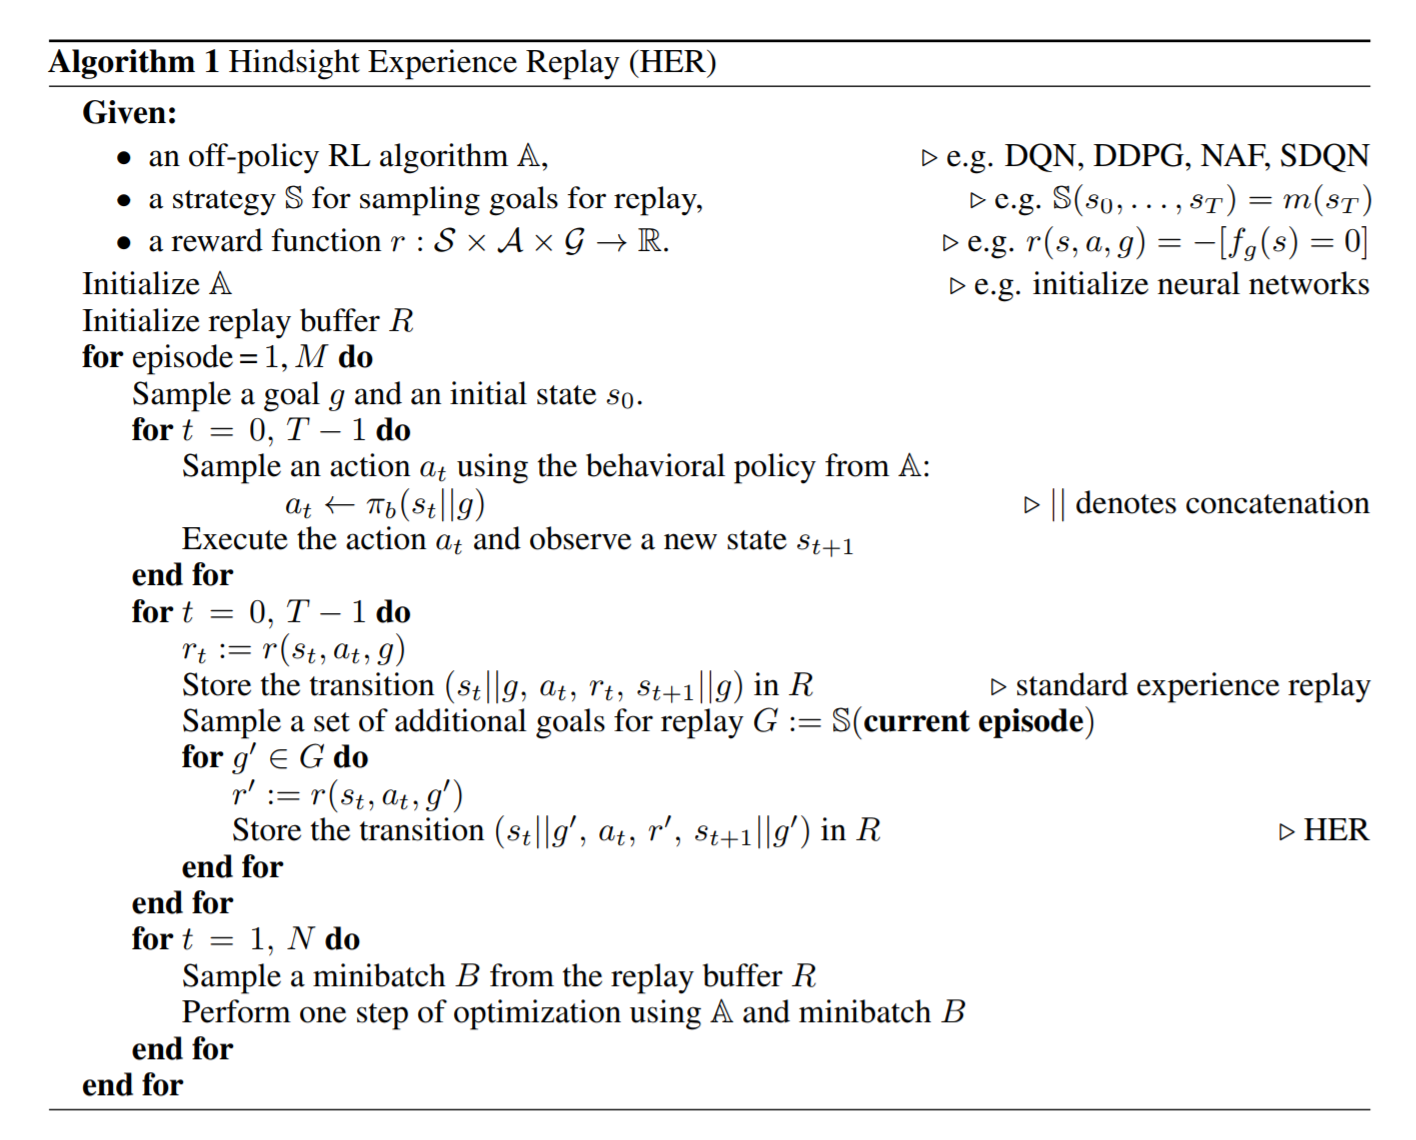
\includegraphics[width=1\textwidth]{her}
    \caption{The hindsight experience replay algorithm presented by \cite{DBLP:journals/corr/AndrychowiczWRS17}.}
    \label{fig:her}
\end{figure}

\begin{enumerate}
\item Describe the hyperparameter settings that you used to train DDPG with HER.  Ideally, these should match the hyperparameters you used in Part 1 so we can isolate the impact of the HER component.
 \begin{solution}
\end{solution}
\item  Plot the learning curve: Every $k$ episodes, freeze the current cloned policy and run 100 test episodes, recording the mean/std of the cumulative reward. Plot the mean cumulative reward $\mu$ on the y-axis with $\pm \sigma$ standard deviation as error-bars vs. the number of training episodes.  Do this on the same axes as the curve from Part 1 so that you can compare the two curves.  
 \begin{solution}
\end{solution}
\item How does the learning curve for DDPG+HER compare to that for DDPG?  What are the limitations of HER?  Give some scenarios in which you would or would not be able to use it to speed up training. 
\begin{solution}
\end{solution}
\end{enumerate}

\section*{General Advice}
\ \\
Due to the more complicated objective function for DDPG, you will likely have to write some of the code in Tensorflow so you have more control over the training procedure.  \href{https://www.tensorflow.org/tutorials/eager/custom_training_walkthrough}{This tutorial} could be useful for you to reference as you are implementing the training procedure for the actor network in DDPG.
%\nocite{*}
\bibliographystyle{plain}
\bibliography{deeprlhw2}

\end{document}

